\documentclass[12pt, letterpaper]{book}
\usepackage{graphicx} %LaTeX package to import graphics
\graphicspath{{../Immagini}} %configuring the graphicx package
\usepackage[T1]{fontenc}
\usepackage[italian]{babel}
\usepackage{hyphenat}
\hyphenation{mate-mati-ca recu-perare}


%Domande:
%1) nei dispositivi che stiamo studiando il body è cortocircuitato con il source? 

% grafici che rappresentano l'andamaneto delle Vth al variare di W e L con i tre metodi 
% 

\begin{document}



\chapter{Estrazione dei paramentri statici}

\section{Tensione di soglia}

La tensione di soglia $V_{th}$ di un transistore MOS è definita come quella tensione tra gate e bulk per la quale la popolazione di minoritari all’interfaccia è uguale alla popolazione di maggioritari nel bulk. Questa definizione non può essere usata direttamente per il calcolo della tensione di soglia dei dispositivi, ma si deve passare attraverso l'analisi delle caratteristiche corrente tensione dai dispositivi. \\	
Per l'estrazione del parametro $V_{th}$ sono stati presi in considerazione vari metodi, in modo da confrontare i risultati di ciascuno e scegliere quale effettivamente usare per lo studio della degradazione delle prestazioni statiche del chip.\\

Il primo metodo analizzato è chiamato \emph{Transconductance Change Method, TCM,} che defiscisce la tensione di soglia come la tensione di gate $V_{GS}$ corrispondente al picco massimo della derivata della transconduttanza $g_m$ rispetto alla tensione di gate ($\frac{dg_m}{dV_ {GS}}$) ed è valido per bassi valori della tensione $V_{DS}$.\\
Questa definizione si basa sul fatto che, quando il dispositivo passa dalla regione di debole inversione alla regione di forte inversione, la dipendenza della corrente di drain ripetto a $V_{GS}$ passa dall'essere esponenziale all'essere quasi constante. 
La transconduttanza è definita come la derivata prima della corrente $I_D$ rispetto alla tensione $V_{GS}$, dunque la derivata della $g_m$ corrisponde alla derivata seconda di $I_D$. Per questo motivo, il massimo di $\frac{dg_m}{dV_{GS}}$ coincide con la tensione alla quale il grafico della corrente passa dalla forma esponenziale a quella quasi constante, ovvero la tensione $V_{GS}+V_{DS}$. Se $V_{DS}$ è piccola, la tensione per la quale la $g_m$ è massima è molto simile a $V_{th}$.\\

\begin{figure}[h!]
\centering
 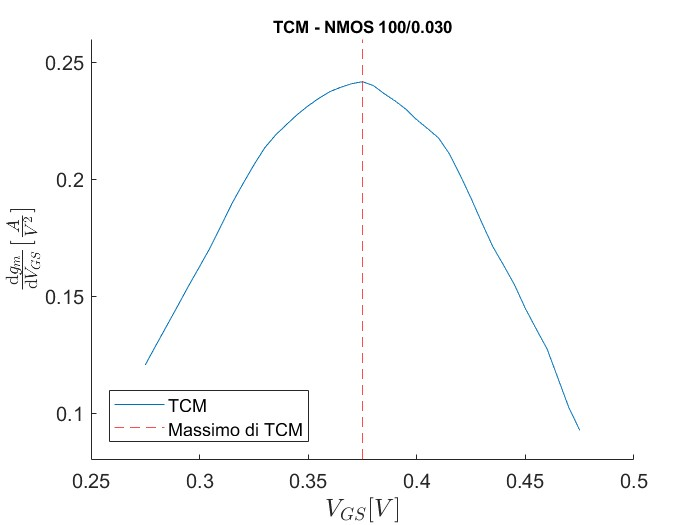
\includegraphics[width=0.49\textwidth]{TCM-N4-100-30-NoFit}
 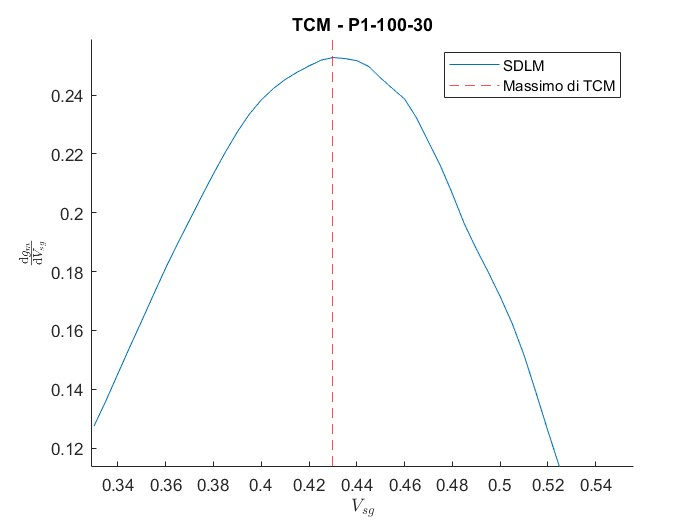
\includegraphics[width=0.49\textwidth]{TCM-P1-100-30-NoFit}
 \caption{Esempio di \emph{TCM} usato su un dispositivo NMOS e un dispositivo PMOS di dimensioni 100-30 a $V_{DS} = 150 mV$}
\end{figure}

Il secondo metodo analizzato è il \emph{Second Difference of the Logarithm of the drain current Minimum method, SDLM}. Questo metodo definisce la $V_{th}$ come la tensione $V_{GS}$ per la quale si ha il picco minimo della derivata seconda del logaritmo naturale di $I_D$ ripetto alla tensione di gate ($\frac{d^2lnI_D}{dV_{GS}^2}$) e vale solo per alti valori di $V_{DS}$. \\

\begin{figure}[h!]
\centering
 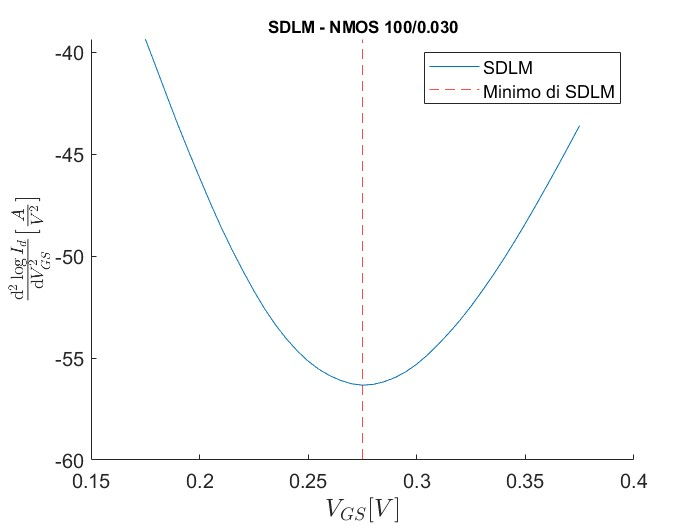
\includegraphics[width=0.49\textwidth]{SDLM-N4-100-30-NoFit}
 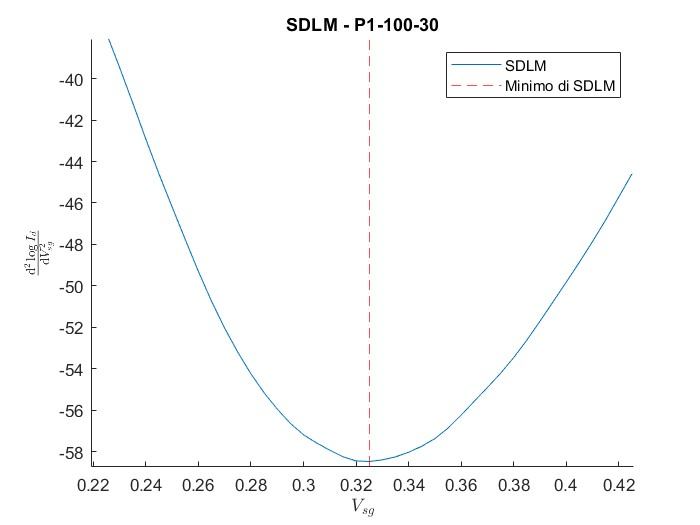
\includegraphics[width=0.49\textwidth]{SDLM-P1-100-30-NoFit}
 \caption{Esempio di \emph{SDLM} usato su un dispositivo NMOS e un dispositivo PMOS di dimensioni 100-30 a $V_{DS} = 900 mV$}
\end{figure}

I due metodi appena esposti, però, sono molto sensibili ai picchi dovuti ad errori di misura e perciò sono difficilmente utlizzabili se prima non si rendono i grafici più puliti. Inoltre, la risoluzione del dispositivo di misura utilizzato e di $5 mV$, il che rende i valori ottenuti della $V_{th}$ molto approssimativi.
Per far fronte a questi due problemi, si è scelto di non tenere conto del minimo e del massimo direttamente ottenuti dalle derivate delle misure fatte, ma di interpolare prima i punti dei grafici ottenuti con una funzione polinomiale e solo a questo punto di prendere in considerazione i picchi di minimo o di massimo. \\

\begin{figure}[h!]
\centering
 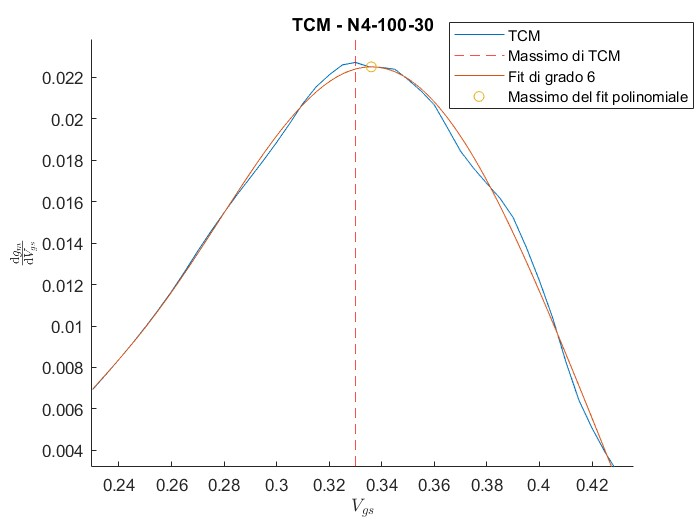
\includegraphics[width=0.49\textwidth]{TCM-N4-100-30}
 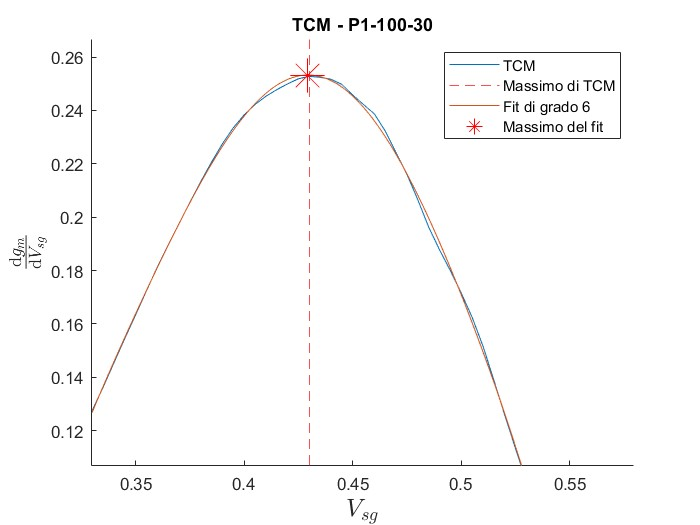
\includegraphics[width=0.49\textwidth]{TCM-P1-100-30}
 \caption{Esempio di \emph{TCM} con fit polinomiale usato su un dispositivo NMOS e un dispositivo PMOS di dimensioni 100-30 a $V_{DS} = 150 mV$}
 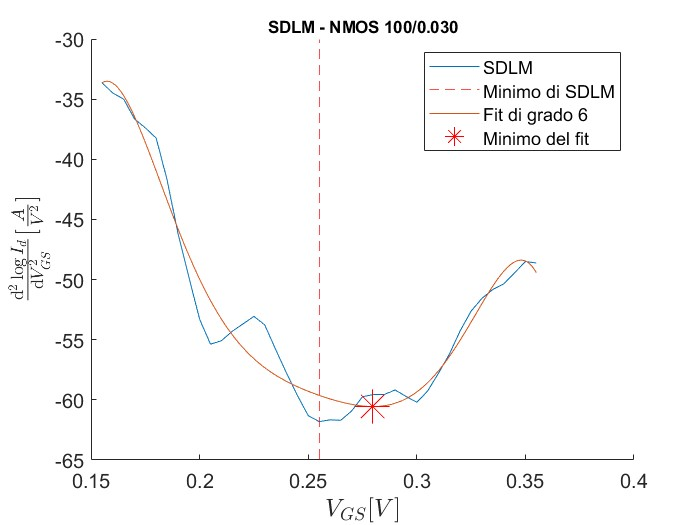
\includegraphics[width=0.49\textwidth]{SDLM-N4-100-30}
 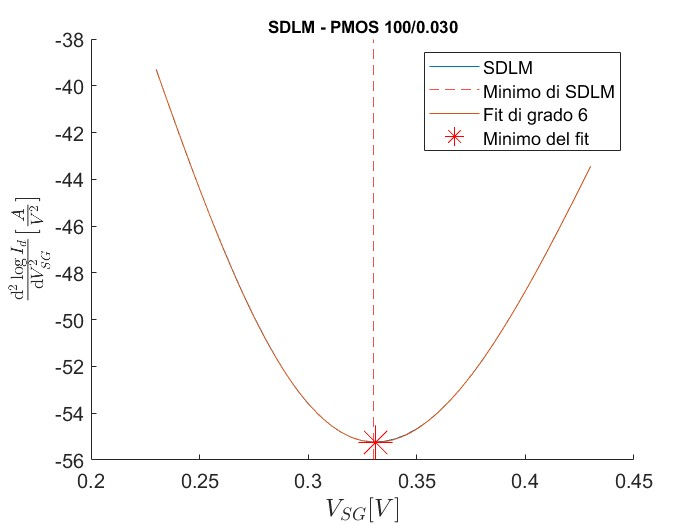
\includegraphics[width=0.49\textwidth]{SDLM-P1-100-30}
 \caption{Esempio di \emph{SDLM} con fit polinomiale usato su un dispositivo NMOS e un dispositivo PMOS di dimensioni 100-30 a $V_{DS} = 900 mV$}
\end{figure}

Per valutare l'accuratezza di questi due metodi si sono quindi calcolate le $V_{th}$ relative ai dispositivi di un PMOS, ottenendo i risultati seguenti:

\begin{center}
\begin{tabular}{| c | c | c |}
\hline
Dispositivo &  $V_{th}$  calcolata con TCM $[mV]$  & $V_{th}$  calcolata con SDLM $[mV]$ \\
 & ($V_{SD} = 150 mV$) & ($V_{SD} = 900 mV$) \\
\hline
100 - 30  & 480.6 & 441.4 \\
100 - 60  & 469.3 & 411.6 \\
200 - 30  & 399.3 & 296.5 \\
200 - 60  & 453.5 & 404.9 \\
200 - 180 & 495.3 & 449.3 \\
600 - 30 & 385.9 & 289.7 \\
600 - 60 & 434.7 & 391.8 \\
600 - 180 & 480.6 & 441.4 \\
\hline

\end{tabular}
\end{center}

In generale i risultati sono abbastanza simili tra le due colonne, per cui si potrebbe prendere in considerazione uno di questi due metodi  per estrarre le tensioni di soglia e studiarne la degradazione.\\
È stato però notato un problema non indifferente: il valore della $V_{th}$ estratta dipende dal grado della funzione polinomiale che interpola i punti delle derivate usate per SDLM e TCM. La differenza dei valori estratti al variare del grado non è molto alta, si parla di pochi millivolt, perciò non influenza considerevolmente il valore della singola estrazione. Questa dipendenza, però, è problematica nel momento in cui si vuole studiare con precisione la degradazione della prestazioni di un dispositivo all'aumentare dell'irraggiamento subito, in quanto piccoli spostamenti del valore di $V_{th}$ dovuti alla scelta arbitraria del grado della polinomiale può far variare eccessiavamente le differenze della misure tra un irraggiamento e l'altro, elemento inaccettabile se si considera che già le misure sono influenzate da errori casuali in fase di misura.\\
Come esempio si riporta il caso della \emph{SDLM} di un PMOS di dimensioni 600-30 con funzione polinomiale interpolatrice di grado 2, 4, 6 e 8. I valori della $V_{th}$ ottenuti sono: 

\begin{center}
\begin{tabular}{| c | c |}
\hline
Grado della polinomiale& $V_{th}[mV]$ \\
\hline
2  & $296.0$ \\
4  & $291.4$ \\
6  & $299.7$ \\
8  & $298.1$ \\
\hline

\end{tabular}
\end{center}

\begin{figure}[h!]
\centering
 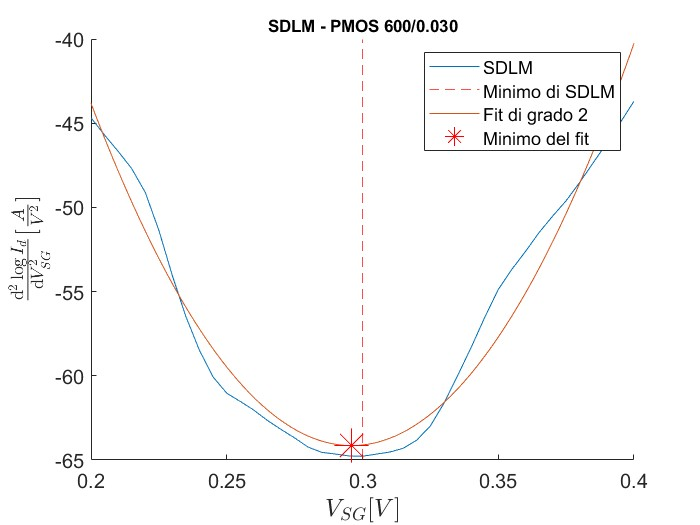
\includegraphics[width=0.49\textwidth]{SDLM-P1-600-30-grado2}
 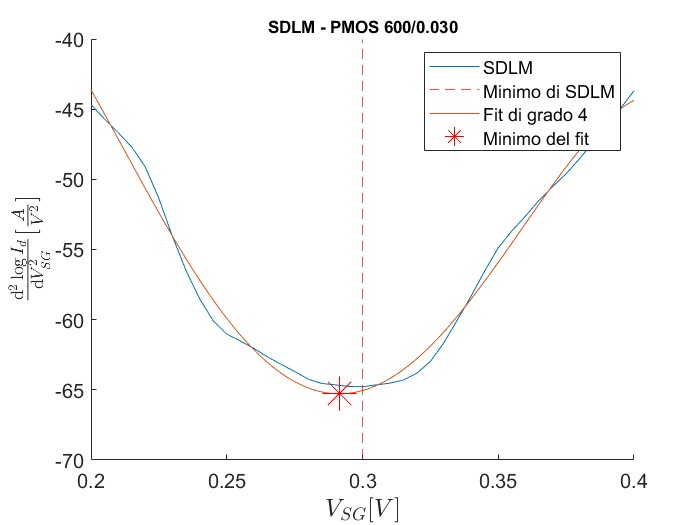
\includegraphics[width=0.49\textwidth]{SDLM-P1-600-30-grado4}
 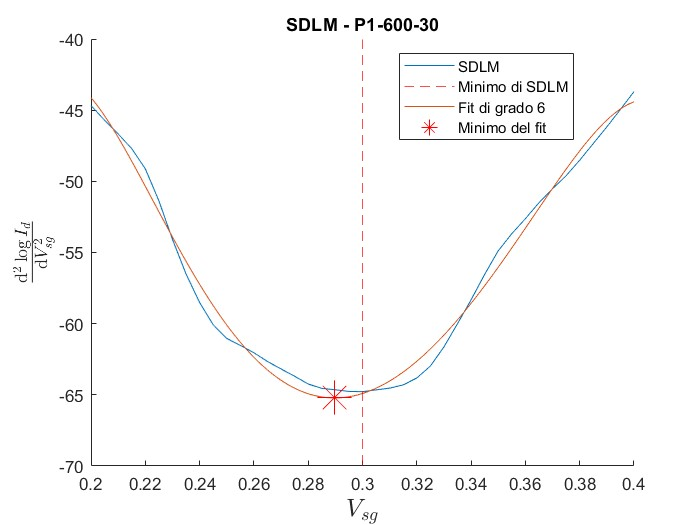
\includegraphics[width=0.49\textwidth]{SDLM-P1-600-30-grado6}
 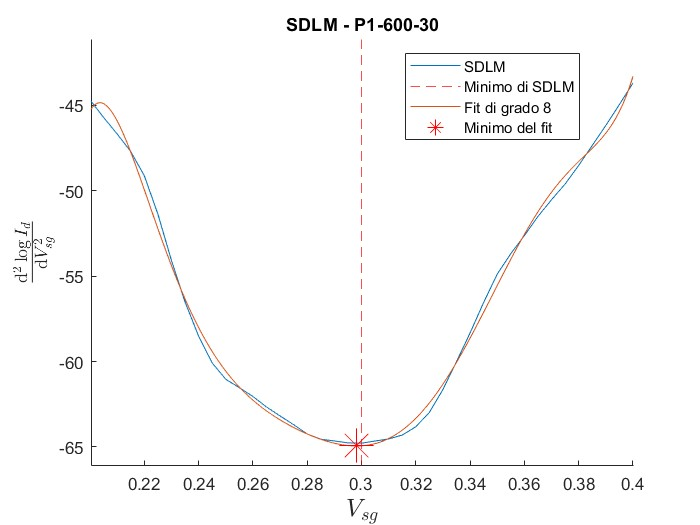
\includegraphics[width=0.49\textwidth]{SDLM-P1-600-30-grado8}
 \caption{Emempi di grafici di \emph{SDLM} su un PMOS di dimensioni 600-30 con fit polinomiale di diversi gradi}
\end{figure}



Per questo motivo si è valutato di utilizzare un terzo metodo: l'\emph{Extrapolation in the Linear Region method, ELR}, con il quale si ottiene la misura della $V_{th}$ attraverso l'analisi della caratteristica $I_D-V_{GS}$.  Tale grafico presenta un punto di flesso attorno al quale il grafico è linearizzabile. Tracciando il fit lineare nell'introno del punto di flesso si ottiene un retta che interseca l'asse delle ascisse, ovvero quello di $V_{GS}$, in un punto il cui valore corrisponde a quello della $V_{th}$.\\


\begin{figure}[h!]
\centering
 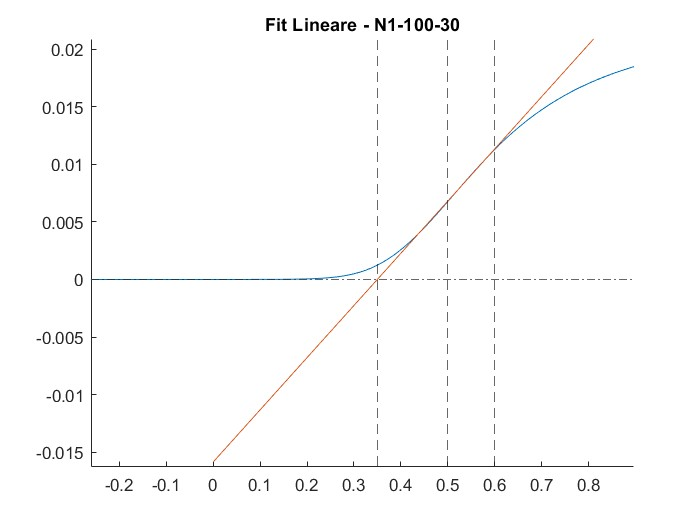
\includegraphics[width=0.49\textwidth]{LinearFit-N1-100-30}
 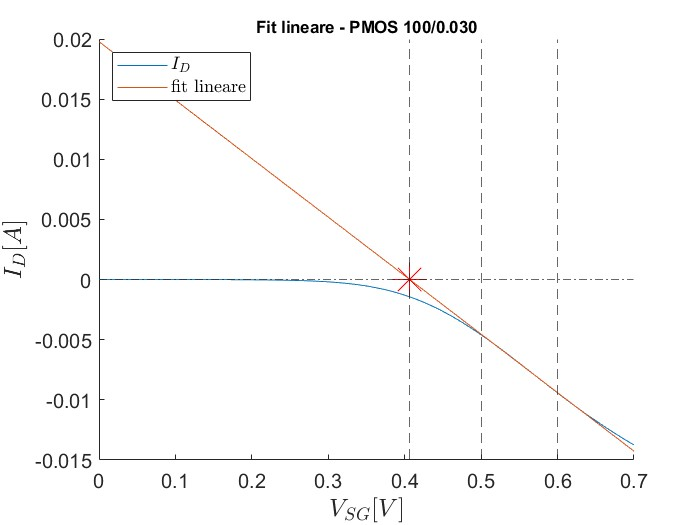
\includegraphics[width=0.49\textwidth]{LinearFit-P1-100-30}
 \caption{Fit lineare della caratteristica  $I_D$-$V_{GS}$ a $V_{DS}=150mV$ di un NMOS e di un PMOS di dimensioni 100-30 nell'intorno $[0,4V ; 0,6V]$ di $V_{GS}$}
\end{figure}

Di per sè, questo metodo è meno preciso di quelli esposti precedentemente, però è più affidabile nella misura delle differenze di $V_{th}$ man mano che i dispositivi vengono irraggiati. problema con le resistenze parassite















\end{document}